\contourlength{1.0pt}
\tikzset{>=latex} % for LaTeX arrow head

\colorlet{xcol}{blue!60!black}
\colorlet{myred}{red!80!black}
\colorlet{myblue}{blue!80!black}
\colorlet{mygreen}{green!40!black}
\colorlet{myorange}{orange!90!black}
\colorlet{mypurple}{red!50!blue!90!black!80}
\colorlet{mydarkred}{myred!80!black}
\colorlet{mydarkblue}{myblue!80!black}
\tikzstyle{xline}=[xcol,thick]
\tikzstyle{width}=[{Latex[length=5,width=3]}-{Latex[length=5,width=3]},thick]
\tikzset{
  traj/.style 2 args={xline,postaction={decorate},decoration={markings,
    mark=at position #1 with {\arrow{<}},
    mark=at position #2 with {\arrow{<}}}
  }
}
\def\tick#1#2{\draw[thick] (#1)++(#2:0.12) --++ (#2-180:0.24)}
\def\N{100} % number of samples

% CIRCLE on axis




% ENERGY vs. t
  \def\A{1.4}
  \def\ang{40}
\def\xmax{6.6} % max x axis
\def\ymax{1.2} % max y axis
\def\om{(2.55*360/(0.94*\xmax))} % angular frequency in degrees

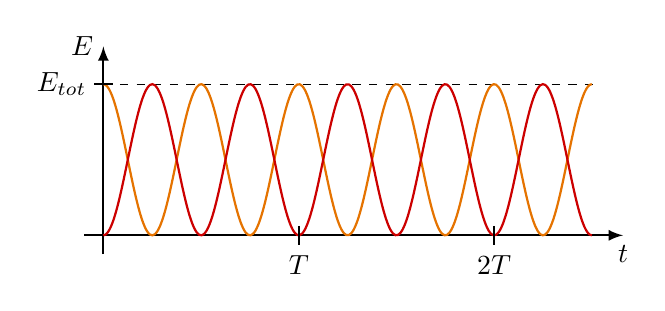
\begin{tikzpicture}
  \def\ymax{2.4} % max y axis
  \def\A{0.8*\ymax} % maximum extension
  \def\om{(2.5*360/(0.94*\xmax))} % angular frequency in degrees
  
  % AXIS
  \draw[->,thick] (0,-0.1*\ymax) -- (0,\ymax) node[left] {$E$};
  \draw[->,thick] (-0.1*\ymax,0) -- (\xmax,0) node[below] {$t$};
  \draw[dashed] (0,\A) -- (0.95*\xmax,\A);
  
  % PLOT
  \draw[xline,myorange,samples=100+\N,smooth,variable=\x,domain=0:0.94*\xmax]
    plot(\x,{\A*cos(\om*\x)^2});
  \draw[xline,myred,samples=100+\N,smooth,variable=\x,domain=0:0.94*\xmax]
    plot(\x,{\A*sin(\om*\x)^2});
  \tick{0,\A}{0} node[left=-1,scale=1] {$E_\text{tot}$};
  \tick{{360/\om},0}{90} node[below,scale=1] {$T$};
  \tick{{720/\om},0}{90} node[below,scale=1] {$2T$};
  
\end{tikzpicture}
